\chapter[Construction d'un détecteur quantique optimal]{Construction d'un détecteur quantique \\ optimal}

On présente ici le détail du problème de la détection optimale quantique avec le critère de l'information mutuelle. Les résultats présentés ici ont fait l'objet d'une proposition de communication à la journée "Traitement du signal et applications quantiques" du GdR CNRS ISIS \cite{engelstein21}.

\section{Formulation du problème}
Le problème de la détection d'état quantique porte sur un ensemble de $m$ états quantiques représentés par les opérateurs densité $\{\rho_j \; , \; 1 \leq j \leq m\}$ munis des probabilités à priori $\{p_j \geq 0 \; , \; 1 \leq j \leq m \}$. L'objectif est d'obtenir un ensemble de $n$ opérateurs de mesure $\{\Pi_k \; , \; 1 \leq k \leq n\}$ permettant d'identifier le mieux possible selon leur probabilités les états d'entrée qui nous arrivent.

En dimension 2, les opérateurs $\rho_j$ et $\Pi_k$ sont des matrices Hermitiennes semi-définies positives, de la forme $\begin{pmatrix}a & b+ic \\ b-ic & d \end{pmatrix}$.

Plusieurs critères ont été proposés à optimiser afin de construire ces détecteurs optimaux. D'une part, on a la possibilité de travailler sur la minimisation de l'erreur quadratique de mesure \cite{Eldar01} ou la maximisation de la probabilité de détection correcte \cite{Eldar03c}. D'autre part, et c'est ce sur quoi nous avons travaillé, on peut considérer le critère de l'information mutuelle entrée-sortie comme critère à maximiser \cite{Davies78}. Il s'agit d'un critère présentant une grande pertinence pour évaluer la transmission d'information sur des canaux de télécommunication. En particulier, l'information mutuelle permet de caractériser le débit maximal d'information qu'il est possible de transmettre sans erreur sur un canal de télécommunication donné.

\medbreak
L'information mutuelle de deux variables aléatoires $X$ et $Y$ a été formulée par Shannon en 1948 \cite{Shannon48}. Elle est donnée en fonction des distributions de probabilité $p_{(X, Y)}(x, y)$, $p_X(x)$ et $p_Y(y)$:

\begin{align}
    I(X;Y) = \displaystyle \sum_{y \in Y} \displaystyle \sum_{x \in X} p_{(X, Y)}(x, y) \log \big(\frac{p_{(X, Y)}(x, y)}{p_X(x) p_Y(y)}\big).
\end{align}

Elle peut aussi être écrite en fonction des entropies des variables aléatoires:

\begin{align}
    I(X; Y) &= H(X) - H(X | Y) \\
            &= H(Y) - H(Y | X) \\
            &= H(X) + H(Y) - H(X, Y).
\end{align}

Avec $H(X)$ entropie marginale de $X$, $H(Y)$ entropie marginale de $Y$, $H(X|Y)$ entropie conditionelle de $X$ sachant $Y$ et enfin $H(X, Y)$ entropie conjointe de $X$ et $Y$. On peut utiliser indifférement $\log_2$, $\log_{10}$ ou $\ln$ pour le logarithme, le changement étant à une constante multiplicative près.

Dans le cas classique, les entropies marginales, conditionnelles et conjointes sont définies par: 

\begin{align}
    H(X) &= -\displaystyle \sum_{x \in X} p_{X}(x) \log(p_{X}(x)) , \\
    H(Y) &= -\displaystyle \sum_{y \in Y} p_{Y}(y) \log(p_{Y}(y)) , \\
    H(X, Y) &= -\displaystyle \sum_{x \in X} \displaystyle \sum_{y \in Y} p_{(X, Y)}(x, y) \log(p_{(X, Y)}(x, y)), \\
    H(Y|X) &= -\displaystyle \sum_{x \in X, y \in Y} p_{(X, Y)}(x, y) \log \big(\frac{p_{(X, Y)}(x, y)}{p_{X}(x)}\big)
\end{align}

Dans le cas quantique, des formules spécifiques existent pour l'entropie d'un état quantique et l'information mutuelle, mais on ne les utilise pas spécifiquement ici. En effet, on s'intéresse à la transmission et récupération d'information classique, sur un canal quantique: on part d'information classique, les $X$, qu'on encode dans les $\rho_j$, pour de la transmition, et on mesure en quantique pour récupérer de l'information classique, les $Y$.

% Dans le cas quantique, les formules restent les mêmes, mais on exprime les probabilités des variables en fonction des valeurs des états quantiques d'entrée.

\medbreak

On a en entrée :

\begin{align}
    P(X = \rho_j) = p_j, \quad 1 \leq j \leq m.
\end{align}

La mesure quantique crée la distribution conditionnelle entrée sortie :

\begin{align}
    P(\Pi_k | X = \rho_j) = \tr(\rho_j \Pi_k) = \alpha_{jk}, \quad 1 \leq k \leq n,
\end{align}

avec $n \neq m$ possiblement. On peut en déduire la distribution de sortie:

\begin{align}
    P(Y = \Pi_k) &= \displaystyle \sum_{j = 1}^{m} P(\Pi_k | X = \rho_j)P(X = \rho_j) \\
    &= \displaystyle \sum_{j = 1}^{m} p_j \alpha_{jk}.
\end{align}

L'entropie de sortie est donc définie par: 

\begin{align}
    H(Y) &= -\displaystyle \sum_{k = 1}^{n} P(Y = \Pi_k) \log(P(Y = \Pi_k)) \\
    &= -\displaystyle \sum_{k = 1}^{n} \big(\displaystyle \sum_{j = 1}^{m} p_j \alpha_{jk}\big) \log\big(\displaystyle \sum_{j = 1}^{m} p_j \alpha_{jk}\big)
\end{align}

L'entropie d'entrée est elle définie par:

\begin{align}
    H(X) &= -\displaystyle \sum_{j = 1}^{m} P(X = \rho_j) \log(P(X = \rho_j)) \\
    &= -\displaystyle \sum_{j = 1}^{m} p_j \log(p_j)
\end{align}

La probabilité conjointe de $X$ et de $Y$ est donnée par: 

\begin{align}
    P(X = \rho_j, Y = \Pi_k) = p_j \tr(\rho_j \Pi_k),
\end{align}

Et donc l'entropie conjointe de $X$ et de $Y$ est donnée par:

\begin{align}
    H(X, Y) = \displaystyle \sum_{j=1}^{m} \displaystyle \sum_{k=1}^{n} p_j \tr(\rho_j \Pi_k).
\end{align}

On obtient donc l'information mutuelle entrée sortie dépendant à la fois des $p_j$ et des $\alpha_{jk}$ :

% On en déduit les probabilités marginales:

% \begin{align}
%     p(X = \rho_i) = \displaystyle \sum_{j}p_i \tr(\rho_i \Pi_j)  \\
%     p(Y = \Pi_j) = \displaystyle \sum_{i}p_i \tr(\rho_i \Pi_j),
% \end{align}

% Et les probabilités conditionelles:

% \begin{align}
%     P(Y=\Pi_j | X=\rho_i) = \frac{\tr(\rho_i \Pi_j)}{\displaystyle \sum_{k} \tr(\rho_i \Pi_k)}
% \end{align}

% L'information mutuelle pour notre problème peut donc être ré-écrite de la façon suivante, en utilisant $\alpha_{jk} = p_j\tr(\rho_j \Pi_k)$ :

\begin{align}
    \label{eq:mi}
    I(\rho; \Pi) &= H(\rho) + H(\Pi) - H(\rho, \Pi) \nonumber \\
    &= - \displaystyle \sum_{j=1}^{m} p_j \log \big( p_j \big) - \displaystyle \sum_{k=1}^{n} \big(\displaystyle \sum_{j=1}^{m} p_j\alpha_{jk} \big) \log \big( \displaystyle \sum_{j=1}^{m} p_j\alpha_{jk}\big) + \displaystyle \sum_{j=1}^{m} \displaystyle \sum_{k=1}^{n} p_j\alpha_{jk} \log( p_j\alpha_{jk} )
\end{align}

On peut aussi exprimer l'information mutuelle en fonction de l'entropie conditionnelle, mais il est plus efficace d'utiliser celle donnée à l'équation \ref{eq:mi} pour la résolution numérique.

Finalement, le problème se formule comme un problème de maximization de l'information mutuelle: on cherche les opérateurs de mesure $\Pi_k$ qui maximisent l'information mutuelle:

\begin{align}
    \max\limits_{\Pi} I(\rho, \Pi)
\end{align}
tel que :

\begin{align}
    \Pi_k \succeq 0, \quad 1 \leq k \leq n \label{eq:contrainte_sdp} \\
    \displaystyle \sum_{k=1}^{n} \Pi_k = I \label{eq:contrainte_somme_id}
\end{align}

La contrainte \ref{eq:contrainte_sdp} qui impose la semi-définie positivité des opérateurs de mesure $\Pi_k$. Enfin, la contrainte \ref{eq:contrainte_somme_id} permet d'obtenir des opérateurs de mesure cohérents pour que les probabilités de mesure $P(\Pi_k)$ soient positives et se somment à 1.

On est en présence d'une fonction non linéaire, convexe, et les contraintes engendrent un ensemble admissible convexe. C'est le cas idéal lors d'une minimisation, mais le problème est une maximisation, de même difficulté qu'une minimisation concave, on ne peut donc pas juste faire une descente de gradient pour le résoudre, l'optimum se situe sur la frontière. On peut utiliser un certain nombre de méthodes approximatives, nous utilisons le calcul par intervalle afin d'obtenir un encadrement global de la solution.

\section{Convexité de l'information mutuelle}
Davies considère dans \cite{Davies78} que l'information mutuelle pour ce problème peut être considérée comme étant convexe, simplifiant la résolution du problème en ayant à chercher le maximum sur les bords. On s'intéresse ici à l'étude de cette convexité.

Dans son article, Davies regroupe les traces et probabilités sous une seule variable $P_{jk} = p_j \tr(\rho_j \Pi_k)$. Ces coefficients $P_{jk}$ forment une matrice des probabilités, telle que :

\begin{align}
    \displaystyle \sum_{jk} P_{jk} = 1, \\
    \displaystyle \sum_{k}  P_{jk} = p_j.
\end{align}
L'information mutuelle s'écrit donc :

\begin{align}
    I(P) = \displaystyle \sum_{j} H(\displaystyle \sum_{k}P_{jk}) + \displaystyle \sum_{k} H(\displaystyle \sum_{j}P_{jk}) -  \displaystyle \sum_{jk} H(P_{jk}) 
\end{align}

La fonction $H(x) = -x \log(x)$ est convexe, et donc $I$ est convexe par rapport à la matrice des probabilités $P$. La figure \ref{fig:mi_convex} illustre cette fonction en fixant $p_1 = 0.3$ et $p_2 = 0.7$.

\begin{figure}[h]
    \centering
    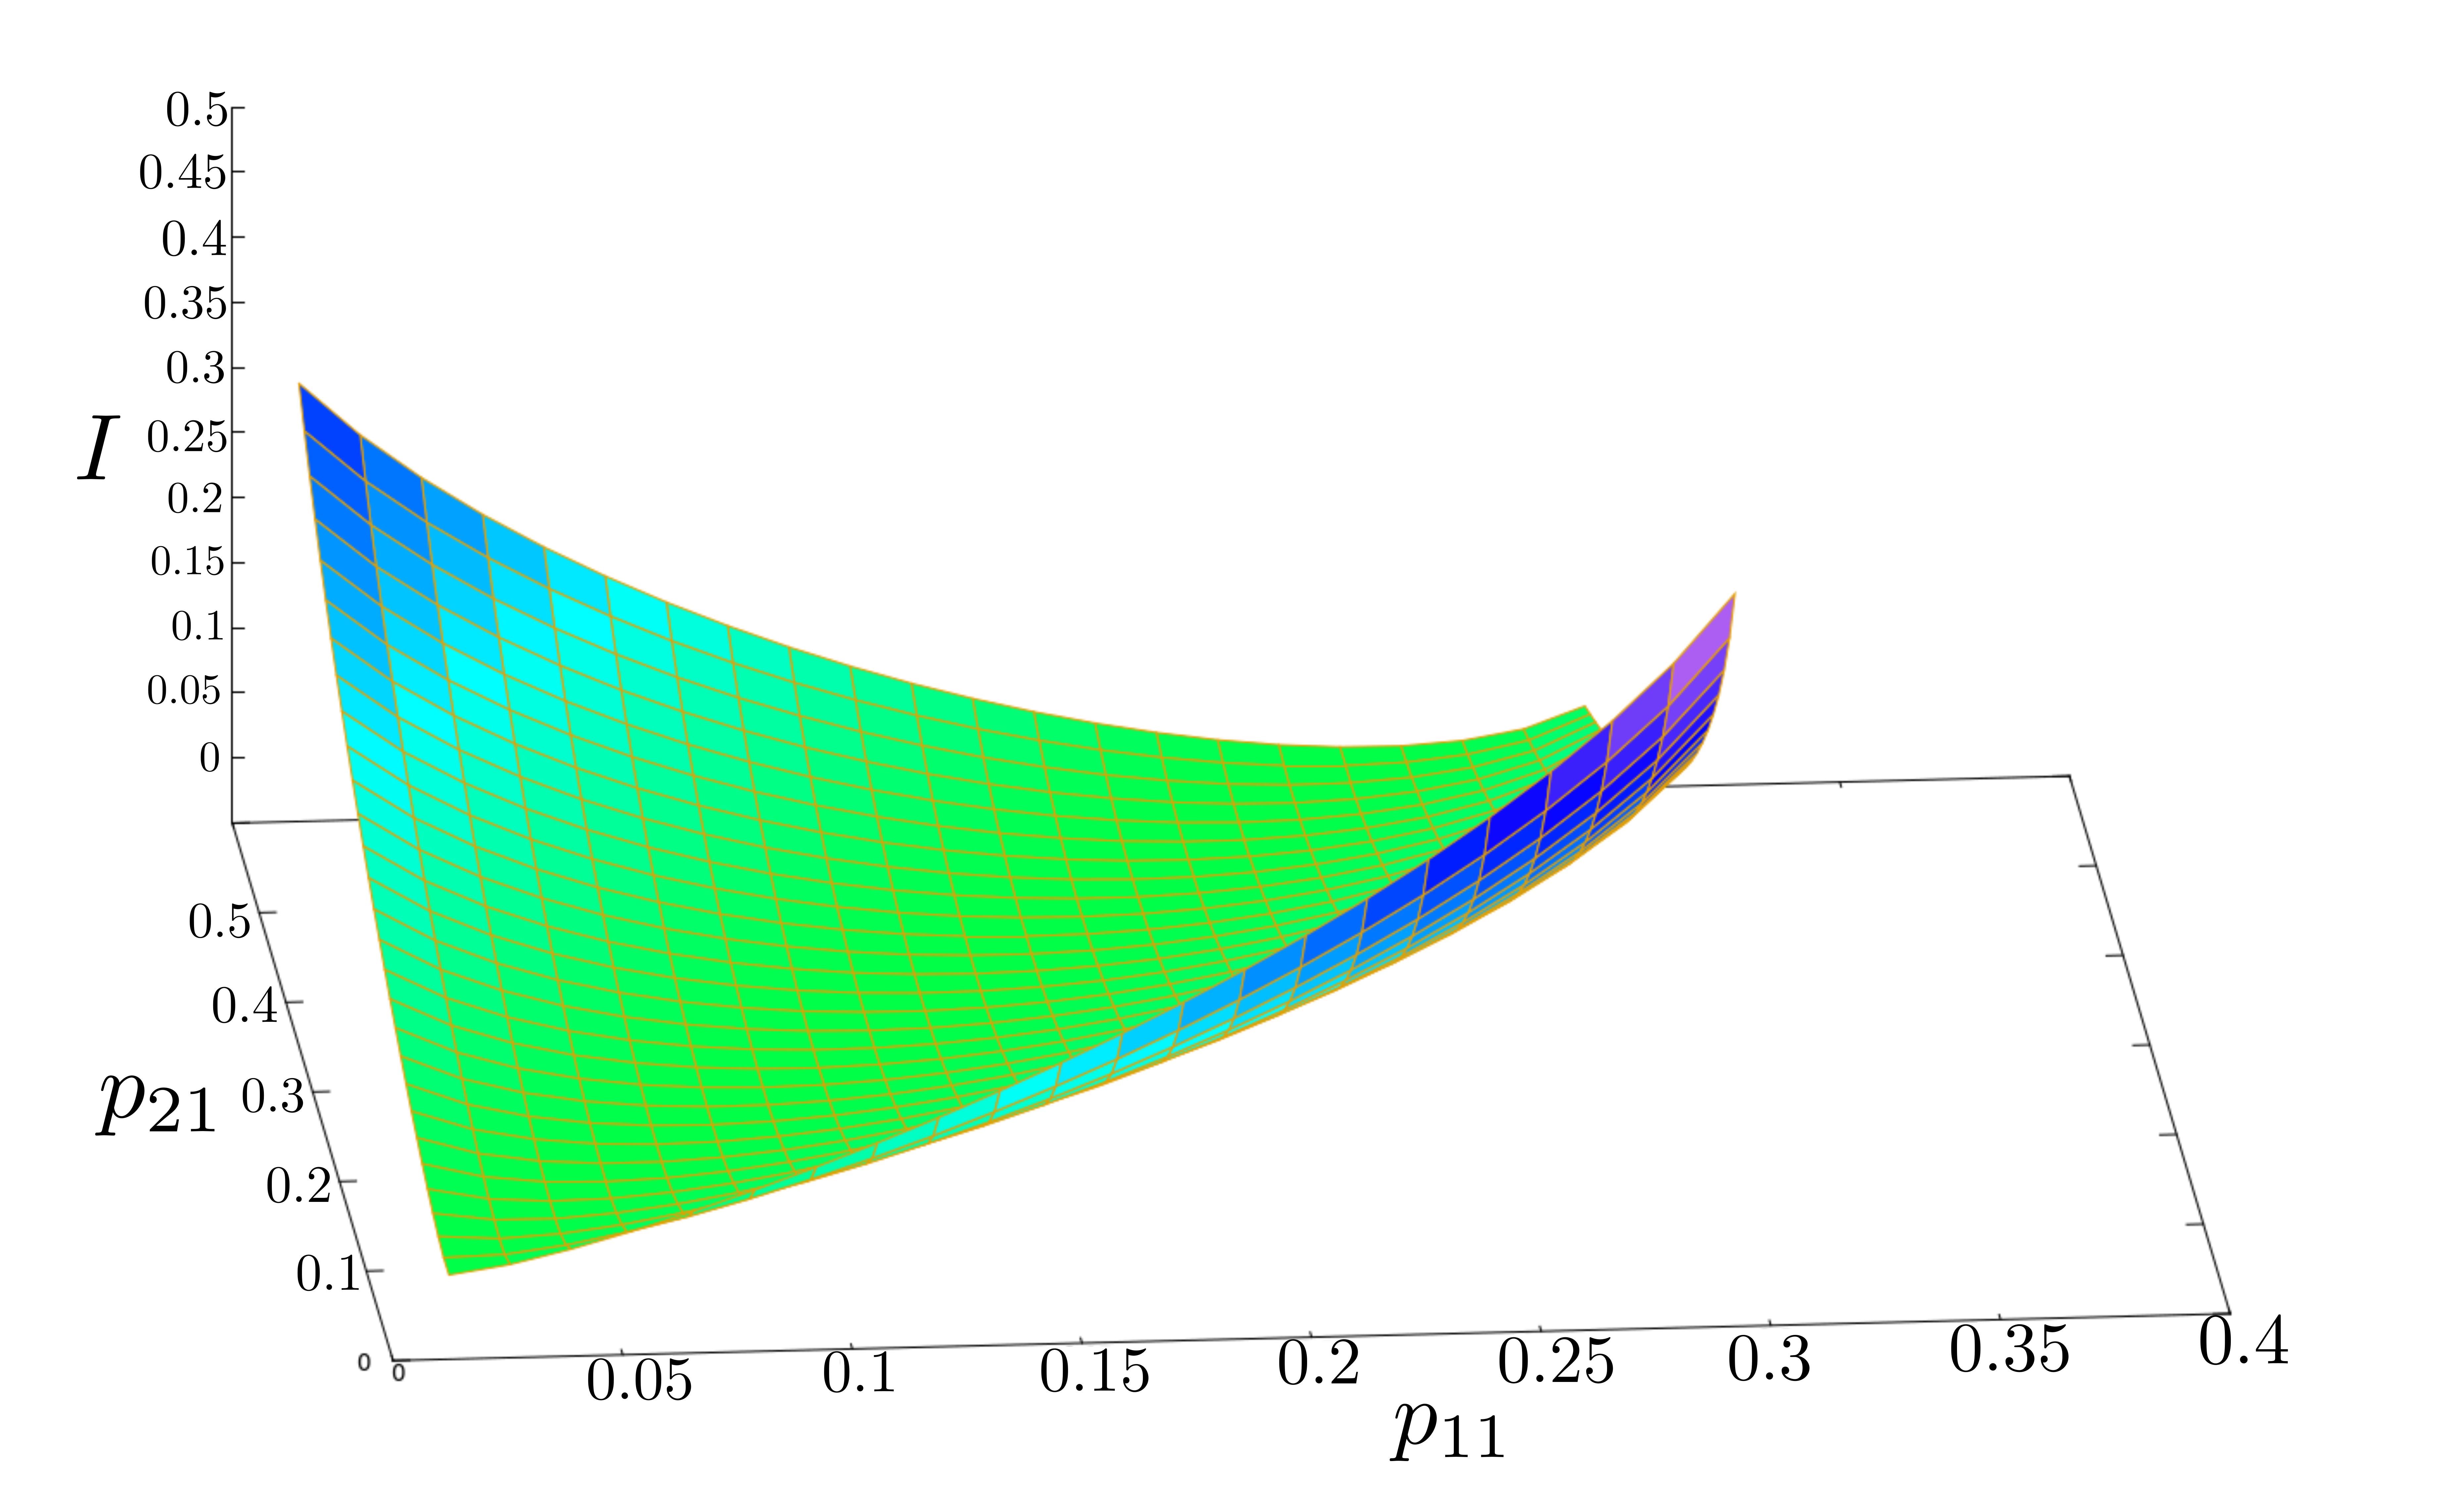
\includegraphics[scale=0.2]{pb/MI_convex.png}
    \caption{Information mutuelle par rapport à la matrice de probabilités}
    \label{fig:mi_convex}
\end{figure}

La convexité semble bien vraie par rapport à $P$, mais on cherche à optimiser les matrices $\Pi_k$. La matrice $P$ comporte les traces de la multiplication $\rho_j \Pi_k$, qui est linéaire par rapport aux coefficients de $\Pi_k$. Si la fonction $I(P)$ est convexe par rapport à $P$, alors elle l'est par rapport aux $\Pi_k$, grace à la linéarité.

Quand on trace la même fonction, mais par rapport aux variables $\Pi_{\alpha_{jk}}$, en se fixant dans un espace deux dimensions, on s'aperçoit que la fonction n'est pas correctement définie sur les bords. Ceci est dû au fait que $x \longrightarrow x\log(x)$ n'est pas défini pour $x < 0$, ce qui fausse ou bloque les calculs, suivant l'implémentation.

\medbreak

\section{Formulation des contraintes}

La définition du problème permet de résoudre notamment les cas immédiats des opérateurs densité $\rho_j$ orthogonaux, mais la résolution devient très lente lorsqu'on passe à d'autres cas non orthogonaux. On rajoute des conditions au problème pour accélérer la résolution.

% Le premier élément à simplifier est l'expression de l'entropie marginale de $X=\rho_j$. En effet, nous l'avons exprimé en fonction de la trace de la multiplication matricielle, mais on peut reprendre la définition donnée lors du cas classique qui dit que $ H(X) = -\displaystyle \sum_{x \in X} p(x) \log(p(x))$. Le problème nous indique que nous connaissons les probabilités préalables des états d'entrée, on peut donc directement exprimer cette entropie en fonction de ces données et donc sans les variables de sortie $\Pi_i$.

Premièrement, on sait que les opérateurs de mesure se somment à l'identité. Cela signifie qu'on peut passer d'un problème à $n$ matrices à un problème à $n-1$ matrices pour $n \geq 2$. Les matrices étant carrées de dimension $N$, on passe de $n \times N^2$ variables à $(n - 1) \times N^2$ variables, ce qui est non négligeable.

De plus, le problème et les contraintes sont symétriques, une permutation des $\Pi_k$ n'influence pas le résultat de la fonction coût. Cela nous permet de couper le problème au moins en deux pour réduire à nouveau le temps de calcul. Du fait de la somme à l'identité, on peut ajouter en contrainte que $\Pi_{1_{1, 1}} \leq \frac{1}{n}$ pour $n$ opérateurs de mesure, puis $\Pi_{2_{1, 1}} \leq \frac{1}{n-1}$, etc.

Ensuite, on peut exprimer la semi-définie positivité des opérateurs de mesure en utilisant le critère de Sylvester. Dans le cas général, il indique que le déterminant de la matrice doit être positif ou nul, ainsi que les $n$ mineurs principaux. Dans le cas à deux dimension, cela se traduit par le déterminant et les deux éléments diagonaux postitifs ou nuls. On a ainsi des contraintes quadratiques sur les entrées.

Enfin, pour rappel, les opérateurs de mesure sont des opérateurs qui ne sont pas nécessairement des projecteurs de rang 1. Pour qu'ils soient de rang 1, il faudrait entre autres que $\tr(\Pi_k) = 1$. On peut considérer qu'on restreint le problème à un cas de rang 1, et dans ce cas rajouter la contrainte que la somme des éléments diagonaux des opérateurs de mesure doit sommer à 1. Cela permet soit de retirer une variable par opérateur de mesure au problème, en l'exprimant par $x_{n+1} = 1 - \displaystyle \sum_{i=1}^{n} x_i$ avec les $x_i$ éléments diagonaux de l'opérateur de mesure, ce qui nécessite une reformulation du problème, soit l'ajout de la contrainte.

\medbreak

% \section{Résolution avec \texttt{ibex}}

% Pour la résolution de ce problème, utilisons la librairie \texttt{ibex} permettant de faire du calcul par intervale, et possède entre autres un outil d'optimisation, \texttt{ibexopt}. Le problème est formulé avec un langage dédié, \texttt{minibex}. Nous avons eu besoin de définir un opérateur additionnel à ceux présents, l'opérateur \texttt{xlog} permettant d'effectuer l'opération $x \times \log(x)$ en redéfinissant $0 \times \log(0) = 0$ pour que les intervalles ne tombent pas à l'infiniquand ils contiennent 0. De plus, \texttt{minibex} ne considère que des problèmes de minimisation, on ré-écrit le problème en prenant la fonction coût opposée : $\max f(x) \Leftrightarrow \min -f(x)$.
% \medbreak
% Le premier test effectué est sur le cas de deux états d'entrée $\ket{\psi_1} = \ket{0}$ et $\ket{\psi_2} = \ket{1}$ ayant pour probabilité respective $p_1 = 0.1$ et $p_2 = 0.9$. Le résultat théorique est connu: les états étant orthogonaux, on doit obtenir les opérateurs de mesure égaux aux opérateurs densité d'entrée. On obtient bien avec \texttt{ibex} les opérateurs suivant:

% $\Pi_1 = \begin{pmatrix} 0 & 0 \\ 0 & 1\end{pmatrix} , \quad \Pi_2 = \begin{pmatrix} 1 & 0 \\ 0 & 0\end{pmatrix},$

% qui correspondent bien à deux opérateurs de mesure orthogonaux. Dans ce cas, l'information mutuelle est comprise dans l'intervalle $I(\rho, \Pi) \in [0.3250, 0.3254]$, avec un temps de calcul de 8.6 millisecondes.
% \medbreak
% Le deuxième cas qu'on peut présenter est le suivant: $\ket{\psi_1} = \ket{0}$ et $\ket{\psi_1} = \ket{+}$ avec comme probabilité respectives $p_1 = 0.1$ et $p_2 = 0.9$. Le résultat théorique n'est pas donné, et on obtient avec \texttt{ibex} le résultat suivant:

% $\Pi_1 = \begin{pmatrix} 0.445 & 0.497 \\ 0.497 & 0.555\end{pmatrix} , \quad \Pi_2 = \begin{pmatrix} 0.555 & -0.497 \\ -0.497 & 0.445\end{pmatrix},$

% avec une information mutuelle comprise dans l'intervalle $I(\rho, \Pi) \in [0.1348, 0.1349]$, et un temps de calcul de 0.79 secondes.

% % On voit bien avec ces deux exemples l'augmentation radicale du temps de calcul quand on passe d'un problème simple, même orthogonal, à un problème plus compliqué.

% En revanche, ibex ralentit fortement dès qu'on sort des cas simples présentés si-dessus, et notament quand on retire la restriction des opérateurs de mesure à des opérateurs densité purs (de trace unitaire). Deux éléments importants sont à l'origine du problème. Tout d'abord, en analysant l'utilisation des ressources cpu lors de la résolution d'un problème, on voit qu'un seul thread est utilisé par \texttt{ibexopt}. Les algorithmes d'optimisation peuvent être parallélisés, et dans le cas de processeurs à plusieurs c\oe urs on pourrait avoir un gain de performance conséquent. Le deuxième élément est en lien avec la convexité de la fonction coût évoqué précédement. On eut alors se limiter aux extremités de la fonction coût pour réduire le nombre de calculs à effectuer. Il faudrait alors implémenter la condition $0 \in [\texttt{grad}]([f])$, ce qui n'est pas prévu de base dans \texttt{ibexopt}.


\pagebreak
\section{Exemple concret}

\subsection{Données du problème}

Considérons deux états purs quantiques:

\begin{align}
    \ket{\psi_1} = \begin{pmatrix}\frac{1}{3} \\{\vrule height 1mm depth 1mm width 0mm}\\ \frac{2 \sqrt{2}}{3}\end{pmatrix} , \quad \ket{\psi_2} = \begin{pmatrix}\frac{1}{\sqrt{2}} \\ {\vrule height 1mm depth 1mm width 0mm} \\ \frac{1}{\sqrt{2}}\end{pmatrix},
\end{align}
avec les probabilités préalables:
\begin{align}
    p_1 &= P(\ket{\psi_1}) = 0.1, \\
    p_2 &= P(\ket{\psi_2}) = 0.9.
\end{align}

Ces deux états peuvent être réécrits sous la forme d'opérateurs densité:

\begin{align}
    \rho_1 = \begin{pmatrix}\frac{1}{9} && \frac{2 \sqrt{2}}{9} \\ {\vrule height 1mm depth 1mm width 0mm} \\ \frac{2 \sqrt{2}}{9} && \frac{8}{9} \end{pmatrix}, \quad \rho_2 = \begin{pmatrix}\frac{1}{2} && \frac{1}{2} \\ {\vrule height 1mm depth 1mm width 0mm} \\ \frac{1}{2} && \frac{1}{2} \end{pmatrix}
\end{align}

% $\rho_1 = \begin{pmatrix}\frac{1}{9} && \frac{2 \sqrt{2}}{9} \\ \frac{2 \sqrt{2}}{9} && \frac{8}{9} \end{pmatrix}$ et $\rho_2 = \begin{pmatrix}\frac{1}{2} && \frac{1}{2} \\ \frac{1}{2} && \frac{1}{2} \end{pmatrix}$.

On a aussi deux opérateurs de mesure inconnus en dimension 2, soit 8 variables inconnues:
\begin{align}
    \Pi_1 &= \begin{pmatrix}a_1 && b_1 + ic_1 \\ b_1 - ic_1 && d_1\end{pmatrix}, \quad \Pi_2 = \begin{pmatrix}a_2 && b_2 + ic_2 \\ b_2 - ic_2 && d_2\end{pmatrix}
\end{align}

On peut déjà calculer l'information mutuelle maximum qui est $H(X)$ \cite{Cover91} puisqu'on a la distribution de probabilités de $X$: 

\begin{align}
    c_{max} = \displaystyle -\sum_j p(X_j) \log_2(p(X_j)) = -0.1\log_2(0.1) - 0.9 \log_2(0.9) = 0.469 \text{ Shannon},
\end{align}

Quelque soient les mesures $\Pi_k$ choisies, on ne pourra pas obtenir une information mutuelle supérieure à $0.469$ qui est l'information maximale en entrée.

On veut résoudre le problème de la maximisation de l'information mutuelle en fonction des $\{\rho\}$ fixés et des $\{\Pi\}$ à ajuster : 

\begin{align}
    &\max\limits_{\Pi_1, \Pi_2} I(\rho_1, \rho_2, \Pi_1, \Pi_2) \\
    % &= -(\tr(\rho_1 . \Pi_1) + \tr(\rho_1 . \Pi_2))\log(\tr(\rho_1 . \Pi_1) + \tr(\rho_1 . \Pi_2)) \\
    % &- (\tr(\rho_2 . \Pi_1) + \tr(\rho_2 . \Pi_2))\log(\tr(\rho_2 . \Pi_1) + \tr(\rho_2 . \Pi_2)) \\
    % &-(\tr(\rho_1 . \Pi_1) + \tr(\rho_2 . \Pi_1))\log(\tr(\rho_1 . \Pi_1) + \tr(\rho_2 . \Pi_1)) \\
    % &- (\tr(\rho_1 . \Pi_2) + \tr(\rho_2 . \Pi_2))\log(\tr(\rho_1 . \Pi_2) + \tr(\rho_2 . \Pi_2))
% 
\Leftrightarrow \max\limits_{\Pi_1, \Pi_2} \big(&-(\alpha_{11} + \alpha_{12})\log(\alpha_{11} + \alpha_{12}) - (\alpha_{21} + \alpha_{22})\log(\alpha_{21} + \alpha_{22}) \nonumber \\
        &- (\alpha_{11} + \alpha_{21})\log(\alpha_{11} + \alpha_{21}) - (\alpha_{12} + \alpha_{22})\log(\alpha_{12} + \alpha_{22}) \nonumber \\
        &+ (\alpha_{11})\log(\alpha_{11}) + (\alpha_{12})\log(\alpha_{12}) + (\alpha_{21})\log(\alpha_{21}) + (\alpha_{22})\log(\alpha_{22}) \big),\nonumber\\
        & \text{avec } \alpha_{jk} = p_j\tr(\rho_j  \Pi_k) ,\nonumber
\end{align}

tel que :

\begin{align}
    \Pi_1 \succeq 0, \Pi_2 \succeq 0,\\
    \Pi_1 + \Pi_2 = I.
\end{align}

On peut réduire considérablement le nombre de variables. En effet, l'équation \ref{eq:contrainte_somme_id} nous indique que les $\{\Pi\}$ se somment à l'identité, on peut donc réécrire $\Pi_2$ en fonction uniquement de $\Pi_1$ pour réduire à 4 variables $\{a_1, b_1, c_1, d_1\}$:

\begin{align}
    \Pi_2 &= I_2 - \Pi_1 = \begin{pmatrix}1 - a_1 && -b_1 - ic_1 \\ -b_1 + ic_1 && 1 - d_1\end{pmatrix}.
\end{align}

Enfin, on voit que dans ce cas particulier les états quantiques d'entrée sont purs et ne comportent aucun terme complexe, ce qui permet immédiatement de retirer le terme $c$ du système puisqu'il ne sera jamais pris en compte. On se retrouve donc au final avec 3 variables $\{a_1, b_1, d_1\}$.

On pose ensuite les contraintes sur ces variables. Tout d'abord, ces variables sont définies sur ces bornes spécifiques: $a_1 \in [0, 0.5]$, $b_1 \in [-1, 1]$, $d_1 \in [0, 1]$. La détermination de la semi-définie positivité passe par les diagonales et le déterminant strictement positifs, d'une part avec les bornes précédentes et d'autre part avec deux nouvelles contraintes sur les 3 variables.
Le problème s'écrit donc :

\begin{align}
    \max\limits_{a_1, b_1, d_1} I(a_1, b_1, d_1) , \nonumber
\end{align}
tel que :
\begin{align}
    &a_1 \in [0, 0.5] , b_1 \in [-1, 1] , d_1 \in [0, 1] , \nonumber \\
    &a_1 \times d_1 - b_1^2 \geq 0 , \nonumber \\
    &(1-a_1) \times (1-d_1) - b_1^2 \geq 0. \nonumber
\end{align}

\subsection{Résolution avec \texttt{ibex}}
On peut tout d'abord résoudre le problème avec \texttt{ibexopt}. C'est un optimiseur garanti sous contraintes, faisant partie de la librairie de calcul par intervalles \texttt{ibex}. Les codes pour la résolution de ce problème sont disponibles en annexe \ref{appendix:ibexopt}. On obtient une information mutuelle de 0.0681 Shannon, avec une précision relative de $1\times10^{-3}$. On obtient les opérateurs de mesure suivant:

$\Pi_1 = \begin{pmatrix} 0.454 & -0.498 \\ -0.498 & 0.546 \end{pmatrix}$, \quad $\Pi_2 = \begin{pmatrix}0.546 & 0.498 \\ 0.498 & 0.454 \end{pmatrix}$,

avec un temps de calcul de $87$ secondes.

Pour la résolution avec \texttt{ibex}, plusieurs modifications et ajouts doivent être faits. Tout d'abord, le langage utilisé par l'outil d'optimisation, \texttt{minibex}, ne considère que les problèmes de minimisation. Cela nécessite simplement de prendre la fonction opposée puisque $\max(f(x)) \Leftrightarrow \min(-f(x))$. On doit ensuite prendre l'opposé de l'intervalle solution pour obtenir le résultat final. Ensuite, le calcul par intervalle fait apparaître une difficulté quant à l'information mutuelle. On se retrouve à avoir de façon répétée des termes du type $x\times\log(x)$. Cette fonction est clairement définie sur $[0, +\infty[$ mais ne l'est pas sur $]-\infty, 0[$. De part le pessimisme du calcul par intervalle, on peut se retrouver à avoir des intervalles complètement négatifs ou contenant $0$ en entrée de la fonction. On se retrouve donc avec un comportement mal défini dans certains cas. La solution pour ibex est de réimplémenter l'opérateur \texttt{xlog} en considérant qu'en dehors ou sur le bord des bornes de définition on considère que la fonction renvoie $0$. 

Un autre point à noter est la grande variabilité des temps de calculs suivant les problèmes qui sont traités.

\subsection{Résolution avec notre optimiseur}
On a rencontré plusieurs problèmes avec ibex qui nous ont poussé à développer notre propre optimiseur. 

Tout d'abord, en étudiant la fonction information mutuelle, on voit que cette fonction est convexe. Cela permet de considérablement réduire l'espace de définition en cherchant le maximum sur le bord de la fonction au lieu de chercher sur toute la fonction. Ceci n'est pas implémenté par défaut sur ibex.

Ensuite, sur l'implémentation de l'algorithme d'optimisation, on peut voir qu'\texttt{ibexopt} n'utilise qu'un seul thread pour son travail. On l'a vu en figure \ref{fig:algomaxim}, la première boucle est facilement parallélisable, ce qui permet d'accélérer considérablement le temps de résolution, et ce en fonction du matériel à disposition.


Enfin, \texttt{ibexopt} ne permet pas l'accès aux boites en place au cours de l'évolution de l'algorithme. Cela ne permet pas une visualisation plus détaillée de ce qui est effectué, quelles régions sont enlevées au fur et à mesure. Dans le cas de problèmes "simples", ce n'est pas forcément important, en revanche avec un problème comme l'information mutuelle, où le comportement en fonction des variables d'entrée n'est pas immédiatement visible, c'est utile pour pouvoir avoir une idée des influences des contraintes. Un exemple de cette visualisation est disponible en figure \ref{fig:visu_dotnet}. Les coordonnées $(x, y, z)$ correspondent aux variables $(a_1, b_1, d_1)$, et les boites sont colorées en fonction des contraintes satisfaites.

Notre optimiseur nous donne les mêmes solutions qu'ibex, à la différence qu'on arrive à une plus grande précision bien plus rapidement, en $13$ secondes pour les mêmes données.

On peut noter entre autres, à la fois sur \texttt{ibexopt} et sur notre optimiseur que les temps de calculs dépendent du problème qu'on a. La figure \ref{fig:temps_optim} montre par exemple que, plus l'angle entre les deux états s'approche de $90$ degrés et des $180$ degrés, qui sont des cas immédiats de problèmes orthogonaux, plus les temps de résolution sont bien moindres.

\begin{figure}[H]
    \centering
    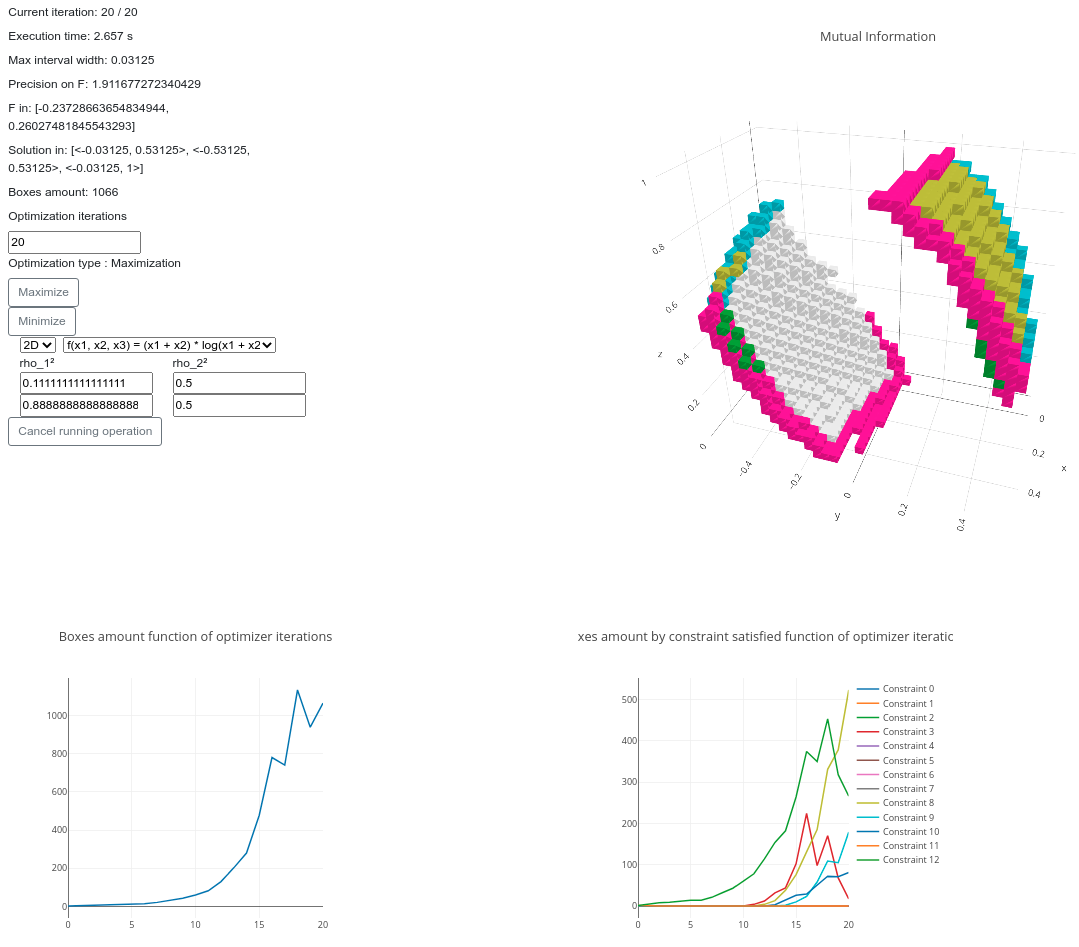
\includegraphics[scale=0.3]{pb/visu_dotnet.png}
    \caption{Interface web de visualisation de l'optimisation}
    \label{fig:visu_dotnet}
\end{figure}

\begin{figure}[H]
    \centering
    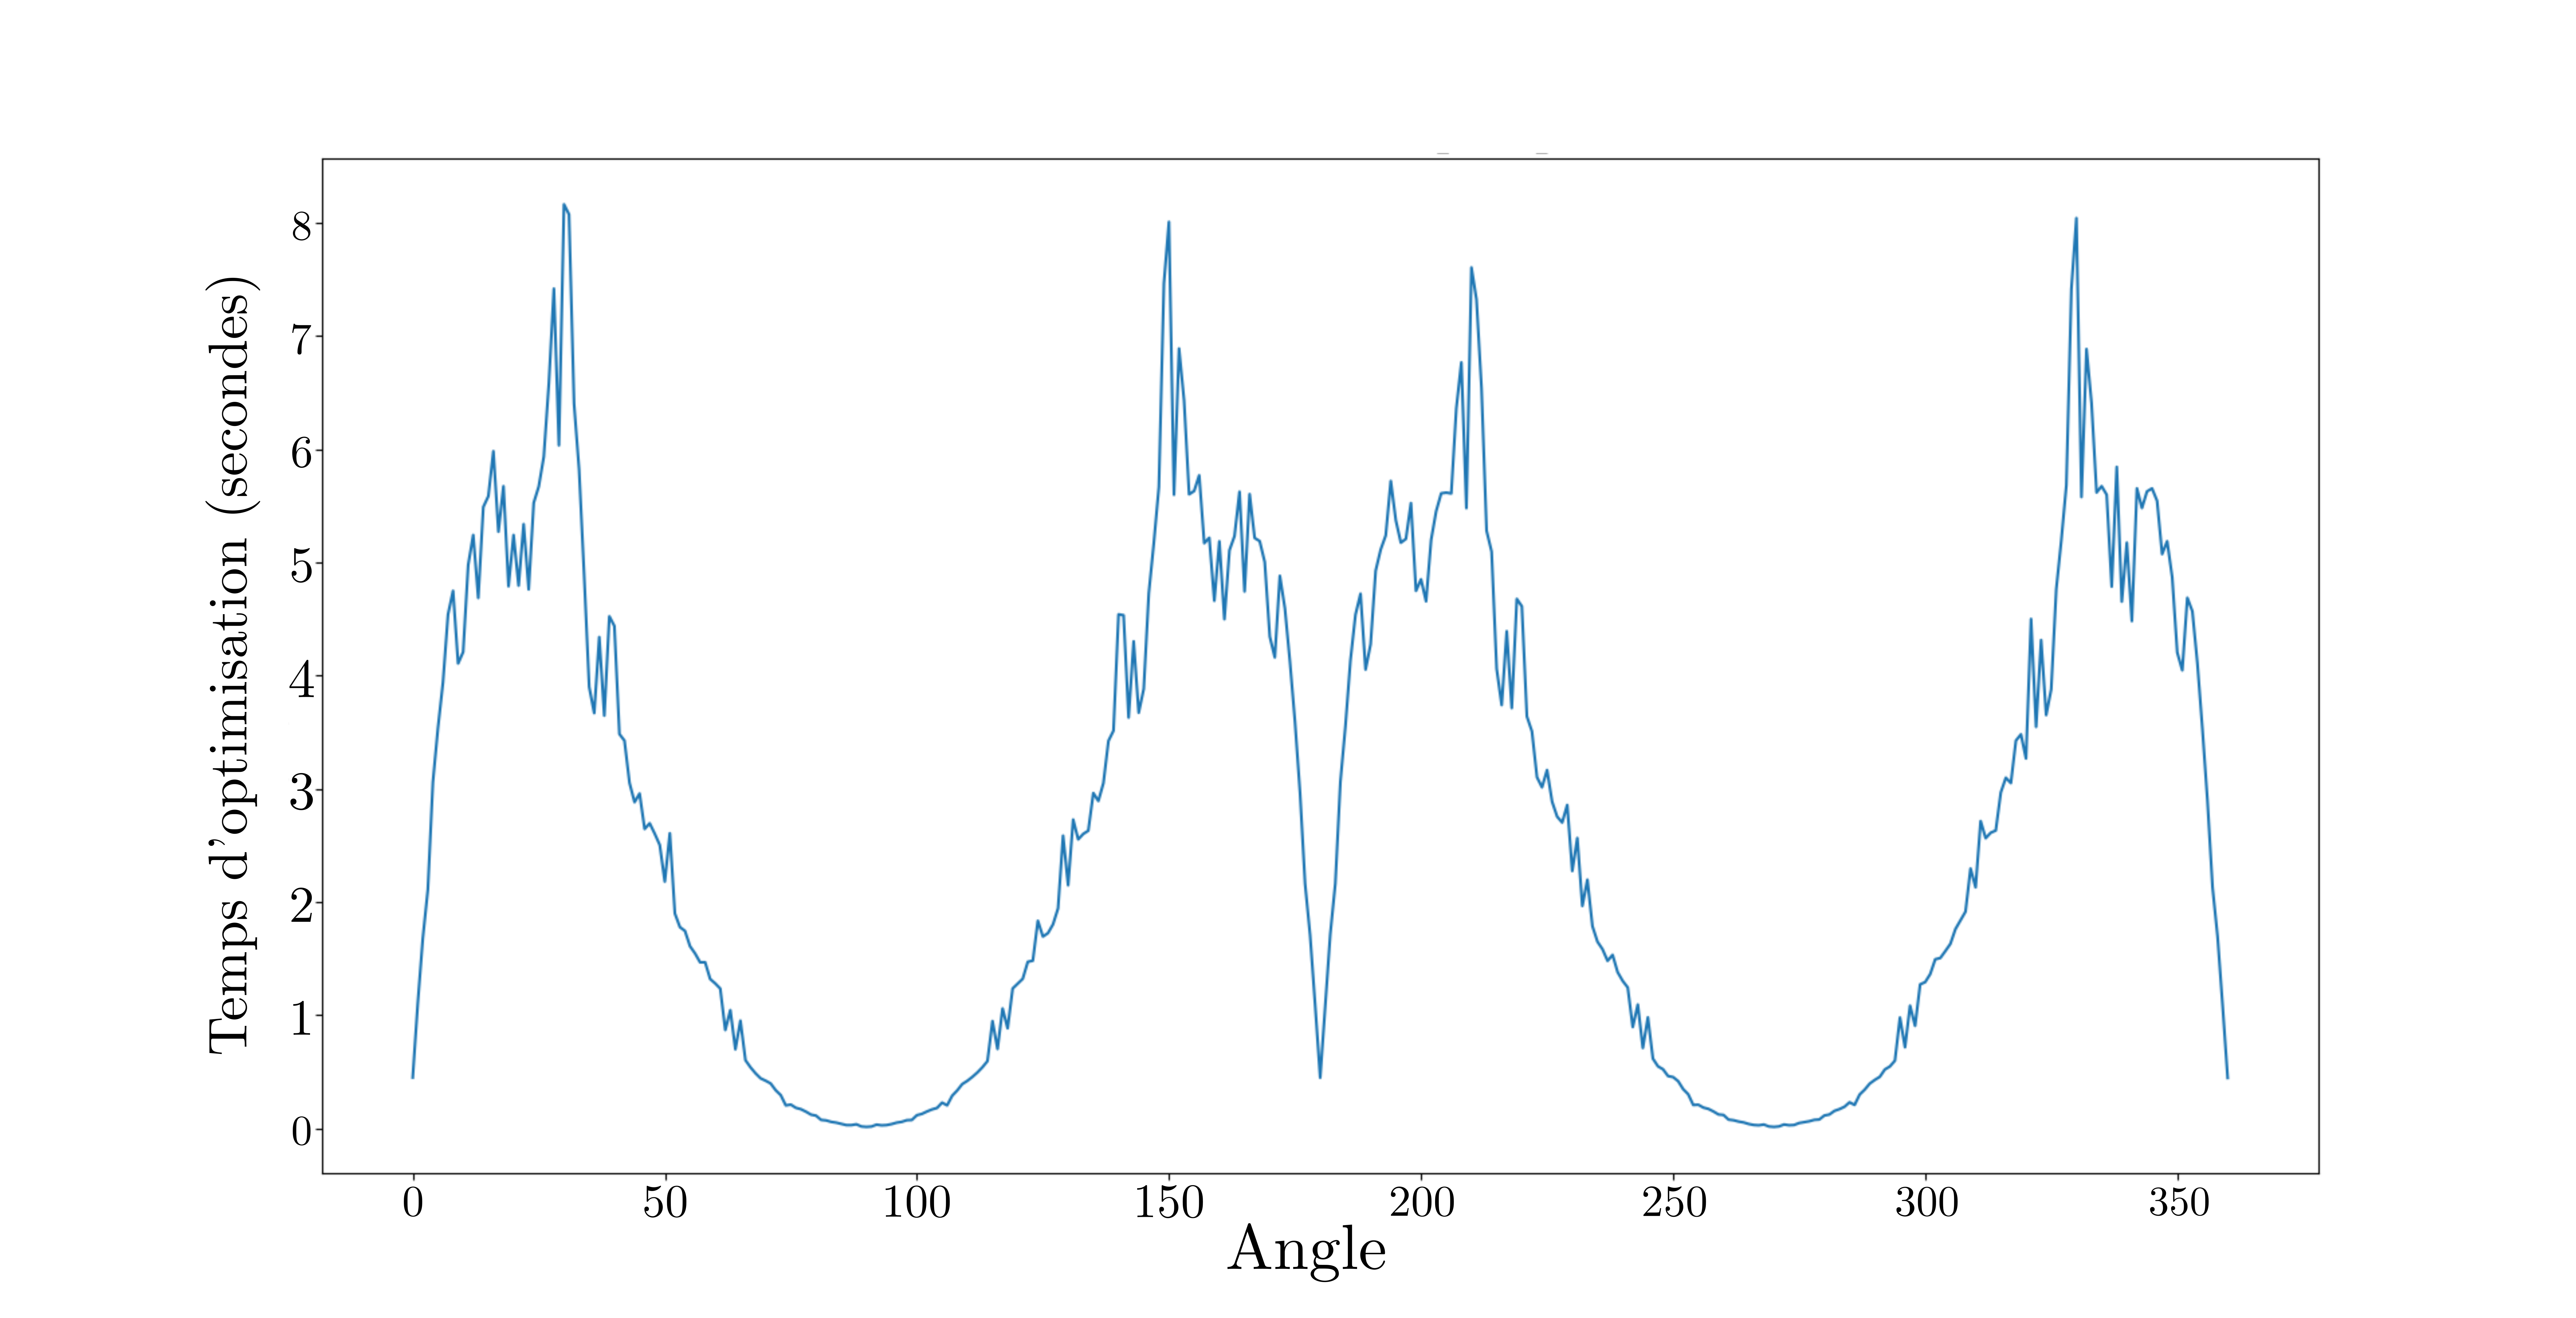
\includegraphics[scale=0.27]{pb/temps_optim.png}
    \caption{Temps d'optimisation en fonction de l'angle entre $\rho_1$ et $\rho_2$}
    \label{fig:temps_optim}
\end{figure}